%%%%%%%%%%%%%%%%%%%%%%%%%%%%%%%%%%%%%%%%%%%%%%%%%%%%%%%%%%%%%%%%%%%%%%%%%%%%%%%%


%\documentclass[letterpaper, 10pt, conference]{IEEEtran}
\documentclass[letterpaper, 10pt, conference]{ieeeconf}
\IEEEoverridecommandlockouts
\overrideIEEEmargins 
\usepackage{tikz}
\usetikzlibrary{calc,decorations.markings,arrows}
\usepackage{tikz-timing}
\usepackage[top=1in,bottom=1in,right=1in,left=1in]{geometry}
\usepackage{amsmath}
\usepackage{xifthen}
\usepackage{amsfonts}
\usepackage{tabu}
\usepackage{graphicx}
\usepackage[font=small]{caption}
\usepackage{subcaption}
\usepackage{cite}
\usepackage{xspace}
\usepackage{subfiles}
\usepackage{url}

% Packages for including pseudo-code
\usepackage{algorithmicx}
\usepackage{algorithm}
\usepackage{algpseudocode}

% Nice Little macro for adding a comment box. Include incrementing comment numbers.
\newcounter{comcount}
\setcounter{comcount}{0}
\newcommand{\mycomment}[1]
{
\refstepcounter{comcount}
\smallskip\noindent\fbox{\parbox{\linewidth}{\emph{Comment \arabic{comcount}} : \small{#1}}} 
}

\newcommand{\spx}{\mathcal{S}}

%
%Once I break this in to multiple sections, each section will be added with:
%	\subfile{filename}
%In those other files, I have as preamble:
%	\documentclass[main.tex]{subfiles}
%

\title{\LARGE \bf
A Stick-Slip Omnidirectional Drive-train for Low-Cost Swarm Robotics: Mechanism, Calibration and Control
}

\author{John Klingner, Nicholas Farrow, Anshul Kanakia, Dustin Reishus and Nikolaus Correll%
\thanks{Department of Computer Science,
University of Colorado at Boulder,
 Boulder, CO 80309,
{\tt\small firstname.lastname{@}colorado.edu}}%
}

\begin{document}
\maketitle


%%%%%%%%%%%%%%%%%%%%%%%%%%%%%%%%%%%%%%%%%%%%%%%%%%%%%%%%%%%%%%%%%%%%%%%%%%%%%%%%
\begin{abstract}
ABSTRACT GOES HERE
\end{abstract}

%\keywords{Swarm robotics, low-cost, hopping robot, bristle-bot principle}


%%%%%%%%%%%%%%%%%%%%%%%%%%%%%%%%%%%%%%%%%%%%%%%%%%%%%%%%%%%%%%%%%%%%%%%%%%%%%%%%
\section{Introduction}
We present a low-cost miniature robot drive-train that approximates omni-directional motion using three vibration motors. Classically, miniature robotic platforms such as r-one \cite{mclurkin2013low}, Jasmine \cite{jasmine} and Alice \cite{alice} require geared motors, which are expensive and difficult to miniaturize. The proposed drive-train is a variant of the ``stick-slip'' actuator that has been introduced in \cite{breguet1998stick}, and has been shown to be particularly attractive for high precision movements \cite{brufau2005micron,chu2006novel,martel2001three,martel2005fundamental,eigoli2012locomotion} and force control \cite{vartholomeos2008analysis}.   

Whereas stick-slip actuators traditionally require to change their length, e.g., using piezo ceramics,  \cite{breguet1998stick, martel2005fundamental}, a similar effect can be achieved using a vibration motor, an effect well known from the ``Bristle-bot'' series of toys. The simplicity and availability of this actuator  has led to its use on low-cost miniature robot platforms such as the Kilobots \cite{rubenstein2012kilobot} based on the design presented in \cite{Vartholomeos2006}, which approximates the dynamics of a differential wheel platform (see also \cite{spartali2013speed} for additional analysis). Achieving fully holonomic motion on the plane requires at least three vibration motors, however. Whereas \cite{Vartholomeos2005} proposes a symmetric three motor design and its analysis, their approach requires all motors to be in phase, which is not feasible on a low-cost platform. This paper addresses these problems by presenting a design, controller and calibration routine that allows omnidirectional motion on a ping-pong ball sized robot ``Droplet'' (Figure \ref{droplets}).

\begin{figure}[h]
	\centering
		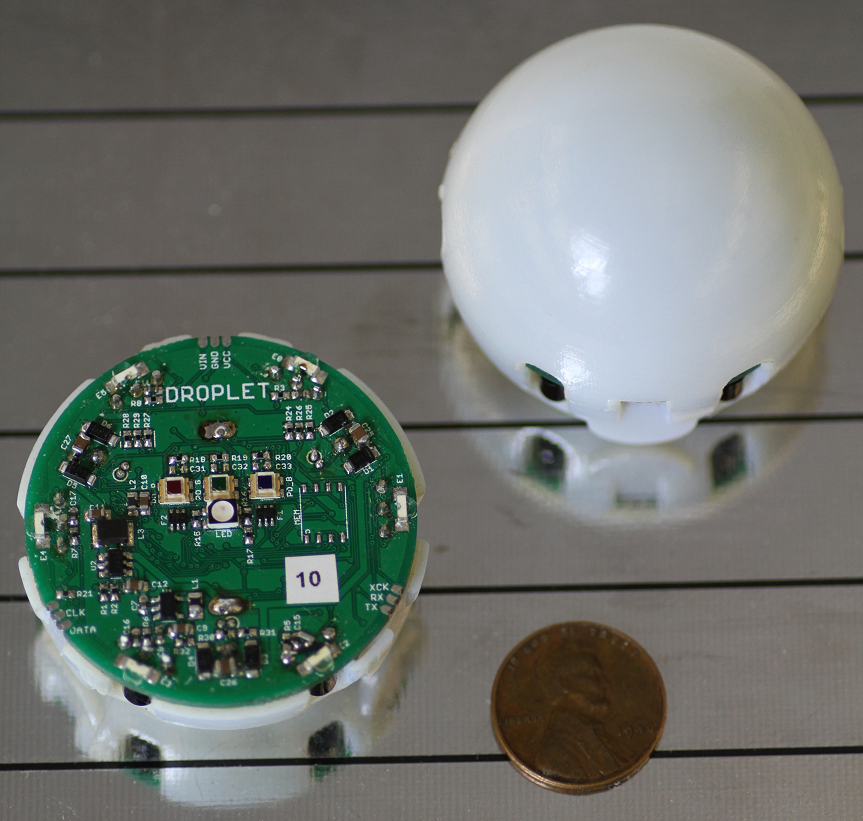
\includegraphics[width=0.8\columnwidth]{./Images/droplets.png}
	\caption{The Droplet swarm robotics platform. Two Droplets are shown, one with the cover removed. A penny is included for scale. The background is the floor of alternating power and ground strips from which the Droplets draw power.}
	\label{droplets}
\end{figure}


%%%%%%%%%%%%%%%%%%%%%%%%%%%%%%%%%%%%%%%%%%%%%%%%%%%%%%%%%%%%%%%%%%%%%%%%%%%%%%%%
\section{The Droplet Swarm Robotic Platform}
The Droplets are an open-source swarm robotic platform, with source code and manufacturing information available online\footnote{\url{https://github.com/correlllab/cu-droplet}}. Their body has a radius of $2.2cm$. They have three extended headers for legs located symmetrically around the robot $1.5cm$ from the center. The Droplets receive power from these legs through a floor with alternating strips of $+5V$ and $GND$. The Droplets use an Atmel Xmega128A3U microcontroller, along with Allegro A3901 Dual Motor Drivers. The motors are a low cost, coin-type model and are mounted symmetrically around the robot opposite the legs, near the outer edge. The motors are oriented such that the axis of rotation moves through the center of the robot and the opposite leg. As locomotion is not their primary intent, the vibration motors used here are inconsistent about both the direction in and frequency with which they spin.

\begin{figure}[h]
	\centering
	\subfile{motorLocations}
	\caption{An image of the Droplet's shell and vibration motors in place. The locations where the legs are mounted are labeled.}
	\label{motorLocations}
\end{figure}

%%%%%%%%%%%%%%%%%%%%%%%%%%%%%%%%%%%%%%%%%%%%%%%%%%%%%%%%%%%%%%%%%%%%%%%%%%%%%%%%
\section{Principle of Operation}

\subsection{Base Motion Principle}
A vibration motor is a DC motor with a mass on the shaft, such that the center of mass is not on the axis of rotation. Spinning the motor throws the mass around, causing motion of the entire motor body due to inertia. As the mass swings through its circular path, the motor experiences a force towards that mass. Over the course of a full rotation, the net force experienced by the motor is 0. This is illustrated in Figure \ref{motorDiagram}.

\begin{figure*}
\centering
\subfile{singleDoFModel}
\caption{Simple 1DoF model of motion principle, from the side.}
\label{motorDiagram}
\end{figure*}

If we neglect friction, the platform will slide backwards and forwards due to the backwards and forwards forces from the mass, but experiences no net translation. With friction, the vertical forces of the mass become relevant. The downward force of gravity is mitigated by the upward force from the swinging mass. Crucially, this means that the total downward force experienced by the platform is lower while the mass is swinging upwards. Thus, the platform experiences reduced friction while the mass is swinging upwards. The direction of lateral magnitude during this period of reduced friction (or, the direction the motor is spinning) determines the direction of travel, see also \cite{Vartholomeos2005,Vartholomeos2006} for a mathematical treatment of this model. Figure~\ref{motorDiagram} illustrates this process. Note that the robot does not actually need to jump up, as long as the upward force sufficiently reduces static friction. 


\subsection{Motion Principle Applied to Droplets}
Combining the 1-DoF actuator described above with others to obtain a 3-DoF robotic platform is not trivial as it requires all motors to be in phase \cite{Vartholomeos2005}, and infeasible with low-cost hardware. Our proposed design deviates from \cite{Vartholomeos2005} by positioning our motors opposite, instead of above, the platform's legs as shown in Figure~\ref{dropletMotorDiagram}. This allows each motor to reduce friction of two legs at a time, letting the platform pivot around the third leg. 

%With the simplifying assumption that the platform is a uniform mass, lets consider the forces applied to the platform as a single motor $m_i$ rotates. Since the platform touches the floor only with its three legs, it will be relevant to consider the downward force $f_i$ on each leg separately.

\begin{figure}
\centering
\subfile{dropletDiagram}
\caption{Arrangement of vibration motors $m_0, m_1$ and $m_2$ and legs $l_0, l_1$ and $l_2$.}
\label{dropletMotorDiagram}
\end{figure}

As the mass on the motor swings upwards, the friction experienced by each leg is reduced. Due to the location of the motor off-center, friction is reduced more for the two legs nearest the motor. The lateral force by the motor -- which is tangent to the platform's circular frame -- thus causes the platform to pivot about the leg opposite it.



\subsubsection{Straight motion}

Let us consider a single pivot caused by motor $i$ ($m_i$), about leg $i$ ($l_i$), of some small, positive radial distance $\theta_i$. This motion causes the center of the Droplet to trace $\theta_i$ of an arc about $l_i$. The length of the chord with the same endpoints as the arc, $C$, i.e. the distance traveled by the center of the Droplet, is given by:
\begin{equation}\label{eq:arclength}
C=2 L \sin\left(\frac{\theta_i}{2}\right)
\end{equation}
Where $L$ is the distance between the robot's center and leg; the radius of the arc. To break this displacement in to its $x$ and $y$ components, we first need to know the angles of the triangle made by the chord and the leg. We can get this using the law of sines:
\begin{equation}
x = \arcsin\left(\frac{L}{C}\sin(\theta)\right) 
\end{equation}
Inserting the arc length $C$ from \ref{eq:arclength} gives:
\begin{align}
x &=\arcsin\left(\frac{L\sin(\theta)}{2 L \sin(\frac{\theta}{2})}\right) \\
\nonumber
   &=\arcsin\left(\cos\left(\frac{\theta}{2}\right)\right)
\end{align}

Given this angle $x$, and the known angle between the Droplet's $x$\~axis and the leg ($\phi_1$), we can calculate the direction of the platform's displacement:

\begin{align}
\delta x_a &= C \cos(\pi - x - \phi)\\
\nonumber
\delta y_a &= C \sin(\pi - x - \phi)
\end{align}

Note also that the orientation of the Droplet has changed by $\theta$. Next, consider a second pivot by $m_2$ of $-\theta$. By symmetry, we now have:

\begin{align}
\delta x_b &= -C\cos(\pi -x -\phi)\\
\nonumber
\delta y_b &= C \sin(\pi - x - \phi)
\end{align}

and the orientation has now changed by $-\theta$, putting the Droplet back in its original orientation. 

In practice, the proposed locomotion scheme only works with one motor being active at a time. In addition to the motor placement that allows pivoting, this assumption allows us to overcome the limitations of the motors being in phase as described in \cite{Vartholomeos2005}. Therefore, the robots are not moving straight, but crawl forward in a S-shape. In order to move straight, this requires an initial turn to counter the offset introduced by the S-shape. The size of this error is a function of $\theta$. As $\theta$ approaches $0$, so does the error. Similarly, when spinning each cycle of three motors doesn't leave us back at our exact original position, but it does bring us pretty close.

%By restricting ourselves to these small-pivot ``steps'', we avoid the requirements of precise balance and motor-phase synchronization that causes trouble with more direct implementations \cite{Vartholomeos2006}.

%To simplify, we focus on the platform moving in one of six directions: (0,180, $+/-$60, $+/-$120) degrees, as well as clockwise and counterclockwise rotation. It should be a straightforward extension to get arbitrary 3DoF motion by combining these directions.

\subsection{Forward and inverse kinematics}
Whereas each pivot motion happens at the maximal speed of the platform, we can approximate the effective speeds $\theta_i$ by introducing delays of varying length after each microscopic pivot. Assuming that low-level control of $\theta_i$ and switching between pivot motions happens much faster than actual motion, we can reduce the proposed mechanism to a circular robot with three standard wheels, albeit without kinematic constraints, at the same location and orientation as the motors shown in Figure \ref{dropletMotorDiagram} and retractable legs. Here, the absence of kinematic constraints lets the standard wheels skid frictionlessly in any direction, whereas the retractable legs allow to enable and disable pivot points, modeling the up and down movements of the platform. 

In this reduced model, each motor $m_0$, $m_1$, and $m_2$ controls the angular velocity $\dot{theta}_0$, $\dot{theta}_1$ and $\dot{theta}_2$ around its associated pivot point opposite of the motor. This lets us derive the following forward kinematic equations in the robot coordinate frame $\dot{x}_r$, $\dot{y}_r$ and $\dot{\theta}_r$.
Here we assume the y-axis to be orthogonal to the spinning direction of motor 2, and the y-axis to to split the angle between the axis connecting motor 1 and leg 1, and the axis connecting motor 0 and leg 0.
\begin{eqnarray}\label{eq:fwd}
\dot{x}_r &=& L\dot{\theta_2}-L\dot{\theta_1}\frac{\sqrt{3}}{2}+L\dot{\theta_0}\frac{\sqrt{3}}{2}\\
\nonumber
\dot{y}_r &=& L\dot{\theta_0}\frac{\sqrt{3}}{2} - L\dot{\theta_1}\frac{\sqrt{3}}{2}\\
\nonumber
\dot{\theta}_r &=& \dot{\theta_0} + \dot{\theta_1} + \dot{\theta_2}
\end{eqnarray}
Here, we assume positive $\theta_i$ to be aligned with the direction of thrust of motor $m_i$ and each leg having distance $l$ from the motors. That is, if all motors spin in the same direction, they all contribute to $\dot{\theta}_r$ in the same way. The fraction $\frac{\sqrt{3}}{2}$ is equivalent from $\cos 30^o$. Notice that motor 2 does not contribute to $\dot{y}_r$ as it spins orthogonally to the y-axis.

Equation \ref{eq:fwd} is a linear system with three unknowns, and we can solve
\begin{eqnarray}
\dot{\theta_2}=\frac{(\dot{x}-\dot{y})}{L}
\end{eqnarray}
and so on.

%%%%%%%%%%%%%%%%%%%%%%%%%%%%%%%%%%%%%%%%%%%%%%%%%%%%%%%%%%%%%%%%%%%%%%%%%%%%%%%%
\section{Experimental platform}
We constructed the ``Droplets'' platform, a ping-pong ball sized, spherical robot with a flat bottom, three legs, three coin-type vibration motors arranged as shown in Figure \ref{dropletMotorDiagram}, and a 6-directional infrared range and bearing system \cite{farrow14}. The legs are spaced 120 degrees apart 15.1mm (0.595in) from the center.

The vibration motors (Hochar) are circular shaped, 10mm in diameter and 2.7mm thick, weigh 1.1g, rated at 3V DC, vibrate at 200$\pm$42 Hz, and of the type commonly used in cell phones and pagers. Although equipped with color-coded wires, the direction of spin is arbitrary and differences in vibration frequency and strength are significant. 

Motors are controlled via an H-Bridge (Allegro A3901) that is driven by a pulse-width modulated (PWM) signal generated by a microcontroller (Atmel Xmega123A3). This setup allows us to provide a series of precise pulses as well as changing the direction of rotation.    

The motors are kept at a a fixed $100\%$ duty cycle. Each step, we turn a motor on for $motorOnTime+offset$, then all motors are off for $motorOffTime$ before the next motor turns on. Figure~\ref{pwmSignals} shows this in more detail. Calibration is done by setting the offset value for each direction of each motor, such that each step causes a pivot of the same magnitude. These offset durations are integers of magnitude $(1/32)^{nd}$ms. For our platform, $motorOnTime$ is $30ms$ and $motorOffTime$ is $40ms$.
\mycomment{Better name than `motorOnTime' would be good and `motorOffTime' and offset would be good.}

\begin{figure}
\centering
\subfile{PWMfigure}
\caption{The PWM signals for motion in the 0 direction. If both forward (FW) and reverse (RV) are high, the motor is braking. If only one signal is high, the motor rotates in that direction. Thus, to spin forward we keep FW high and drop RV low when we want the motor to actually spin.}
\label{fig:pwmSignals}
\end{figure}
\mycomment{Planning on adding more to PWM diagram.}


\begin{figure}[h]
	\centering
	\subfile{motorLocations}
	\caption{An image of the Droplet's shell and vibration motors in place. The locations where the legs are mounted are labeled.}
	\label{fig:PWMs}
\end{figure}

%%%%%%%%%%%%%%%%%%%%%%%%%%%%%%%%%%%%%%%%%%%%%%%%%%%%%%%%%%%%%%%%%%%%%%%%%%%%%%%%
\section{Auto-Calibration}
Additional challenges arising from low-cost hardware is that achieving equal step sizes requires tedious calibration.
It is possible to calibrate each platform manually, by setting values and eyeballing how well they work. As stated earlier, however, this platform is motivated by a desire for low-cost, large scale robot swarms.  Manual calibration of a swarm of thousands of robots would be completely impractical, and so we automate the process.

\subsection{Experimental Setup}
Data is collected using a high resolution USB camera\footnote{Microsoft LifeCam Cinema}, and RoboRealm \cite{RoboRealm}. A fiducial marking is taped to the top of the platform to aid in tracking and orientation calculations. Specifically, we collect the position (x,y coordinate) and orientation of the Droplet in each frame.

To update the Droplet's calibration settings, we find the least-squares best-fit circle of the collected coordinates. Specifically, the circle's radius and whether it is on the Droplet's left or right. While calibrating for walking straight, we optimize for maximizing the radius of the fitted circle (if the Droplet travelled perfectly straight, the radius would by infinite). While calibrating for spinning, we optimize for minimizing the radius of the fitted circle (a perfect spin would have radius 0).

We communicate with and control the platform through a serial to IR transmitter. 

\mycomment{Image of experiment setup here would be nice.}


\subsection{Calibration Method}
\begin{algorithm}
\caption{Automated method for calibrating an individual Droplet's rotational motion}
\begin{algorithmic}
	\Function{Auto\_Calibrate}{$dir, \alpha, \beta$}		
		\State $\spx \gets$ init\_simplex\_guess()
		\State $[\mu^*_1,\mu^*_2, \mu^*_3] \gets$ Nelder\_Mead($\spx, dir, \alpha, \beta$) 
		\State write\_to\_memory($id_{robot}, dir, \mu^*_1,\mu^*_2, \mu^*_3$)
	\EndFunction
	\Function{Nelder\_Mead}{$\spx, dir, \alpha, \beta$}
		\State $radii \gets$ new list()
		\State $v \gets$ new list()
		\For{$\vec{\mu}$ in $\spx$}
			\State $radii$.push(get\_robot\_spin\_circle\_est($\vec{\mu}, dir$))
			\State $v$.push(get\_robot\_spin\_vel\_est($\vec{\mu}$))
		\EndFor
		\State $\spx' \gets$ new\_simplex\_est($\spx, radii, v, dir, \alpha, \beta$)
		\If{within\_tolerence($\spx', radii, v$)}
			\State \Return best\_values($\spx'$)
		\Else
			\State Nelder\_Mead($\spx', \alpha, \beta$)
		\EndIf
	\EndFunction
\end{algorithmic}\label{alg:spx}
\end{algorithm}

We use the popular Nelder-Mead Simplex algorithm \cite{NelderMead} to calibrate motor parameters for spinning in a given direction (clockwise or anti-clockwise), as seen in Alg.(\ref{alg:spx}). 

The simplex algorithm attempts to minimize the radius of the circle that the droplet makes while rotating while, at the same time, maximize the speed of rotation. The objective function used by the algorithm is,
\begin{equation}
\text{(max.)} \quad -\alpha.r_{circ}(\mu_1, \mu_2, \mu_3) + \beta.v_{rot}(\mu_1, \mu_2, \mu_3)\label{eq:maxcal}
\end{equation}
where $\alpha$ and $\beta$ are weighting constants such that $\alpha > \beta$, as we prefer motor values that minimize circle radius over rotational speed.

Each of the four vertices in the simplex is a set of three motor calibration parameters, i.e., $\spx = \{\vec{\mu^1}, \vec{\mu^2}, \vec{\mu^3}, \vec{\mu^4}\}$, where $\vec{\mu^i} = \{\mu^i_1, \mu^i_2, \mu^i_3\}$. The algorithm attempts to provide iteratively better motor control parameters by solving the optimization problem \eqref{eq:maxcal} till a sufficiently accurate set of parameters is provided that falls within the desired tolerances of rotational circle radius and velocity.

Two factors effect the radius the Droplet traces while attempting to spin: uneven step size and overall step size. If the step sizes are uneven, then the Droplet won't trace a true circle. When the step sizes are even, then the error in
The reader should note that a solution provided by the Nelder\_Mead() algorithm is not unique. Since the circle radius is minimized when all three motors are the s

, i.e., there are multiple valid sets of motor values, $\mu_i$, that minimize circle radius. As long as all pivots are of the same magnitude, this just gives one of them.
\mycomment{Not sure what that last sentence means.}

Additionally, this method identifies which motors are `flipped'---i.e., which motors spin opposite from what's expected. This is because having the motor directions wrong results in a large radius.

It's possible that Nelder-Mead will find a CCW spin, with all motors flipped. After the algorithm comes to a stop, the mean change in orientation is checked to verify that the spin direction is correct. The rest of the procedure only requires that one direction of spin be optimized; it does not care which.

Once we have clockwise spin calibrated, this is equivalent to having three matched pivot sizes for the motors' clockwise spins. To finish calibrating, we just need to find counterclockwise values that match the clockwise ones.

This is done for each motor independently by having the Droplet walk straight in a direction. Now, we want to maximize the radius of the the circle traced by the Droplet. As the droplet improves straight-line motion accuracy, the radius of the circle transcribed by its motion approaches $\infty$. Changes in calibration values are made proportional to circle radius until we've reached the limits imposed by the resolution of our calibration value.

Simply calibrating for CW and then CCW spin doesn't work because it gives two sets of pivot magnitudes, one for CW and one for CCW rotation. Each set is matched with the other pivots in its set, but without additional information we have no information about the comparative magnitudes across the sets.

%%%%%%%%%%%%%%%%%%%%%%%%%%%%%%%%%%%%%%%%%%%%%%%%%%%%%%%%%%%%%%%%%%%%%%%%%%%%%%%%
\section{Results}

What are the experiments that we have done to show that this works? All plots here.

\begin{figure}
\centering
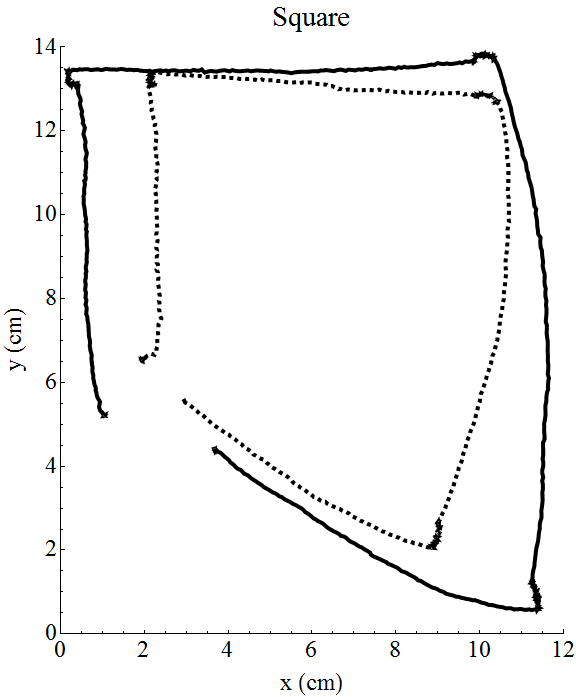
\includegraphics[width=\linewidth]{Images/dropletWalksSquare}
\caption{Two attempts (solid, dashed) of a calibrated Droplet walking in a square, combing straight motion with a rotation.}
\label{fig:squareExperiment}
\end{figure}

\begin{figure}
\centering
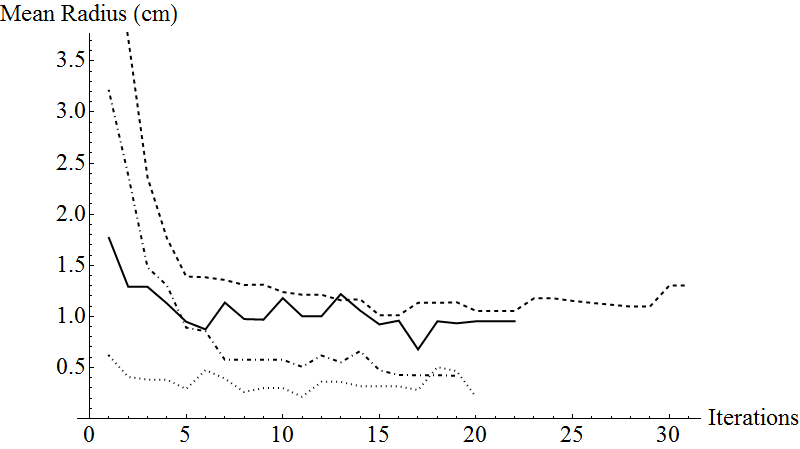
\includegraphics[width=\linewidth]{Images/radiiConverging.png}
\caption{The mean of the best three points of the simplex after each pass through the Nelder-Mead optimization loop, shown for four different Droplets. After the optimization converges or a particularly good value is found, the motors are set to the best of all settings tested.}
\label{fig:radiiConverging}
\end{figure}
\begin{figure}
\centering
\begin{tabular}{r|c|c|c|c|c|c}
 ID & $m_0$ & $-m_0$ & $m_1$ & $-m_1$ & $m_2$ & $-m_2$ \\
\hline
15 & 68 & -1 & 56 & -5 & \emph{40} & \emph{0}\\ 
18 & 84 & -89 & 84 & 202 & \emph{128}  & \emph{290}\\
\end{tabular}
\caption{Sample of calibrated values for specific Droplets. \emph{Italicized} values indicate that that particular motor was flipped. $-m$ is used to indicate the reverse value for that motor.}
\label{dropletValueTable}
\end{figure}

\mycomment{Going to be adding at least a couple more droplets to that table, hopefully!}

%%%%%%%%%%%%%%%%%%%%%%%%%%%%%%%%%%%%%%%%%%%%%%%%%%%%%%%%%%%%%%%%%%%%%%%%%%%%%%%%
\section{Discussion}
Ditch the whole computer vision set up and use the Droplet's IR communication and range and bearing powers to get data and have the swarm calibrate itself.

Get arbitrary 3DoF motion by combining directions.

\section{Conclusion}
To make an analogy to animal strides, the Droplets are only capable of strides in which one leg is ``in the air'' at a time. Any more than that and the Droplet becomes unstable.

Conclusory stuff here.

\section*{Acknowledgments}
This work has been supported by NSF award \#1150223 and a CI fellowship to D. Reishus.


\bibliographystyle{ieeetr}
\bibliography{mybibfile}

\end{document}

